\documentclass[12pt]{article}
\usepackage{url,graphicx,tabularx,array,geometry}
\usepackage{listings}
\usepackage[utf8]{inputenc}
\usepackage{setspace}
\usepackage{amsmath}
\usepackage{enumitem}
\setlength{\parskip}{1ex} %--skip lines between paragraphs
\setlength{\parindent}{0pt} %--don't indent paragraphs

%-- Commands for header
\renewcommand{\title}[1]{\textbf{#1}\\}
\renewcommand{\line}{\begin{tabularx}{\textwidth}{X>{\raggedleft}X}\hline\\\end{tabularx}\\[-0.5cm]}
\newcommand{\leftright}[2]{\begin{tabularx}{\textwidth}{X>{\raggedleft}X}#1%
& #2\\\end{tabularx}\\[-0.5cm]}

\onehalfspacing
%\linespread{2} %-- Uncomment for Double Space
\begin{document}

\title{Imperative and System Programming Autumn 2013}
\line
\leftright{\today}{Alexander Rüedlinger, 08-129-710, Group 05} %-- left and right positions in the header
\section*{Series 6}

\subsection*{1. Pointers, Arrays and Stack segments}
\begin{figure}[!htb]
\centering
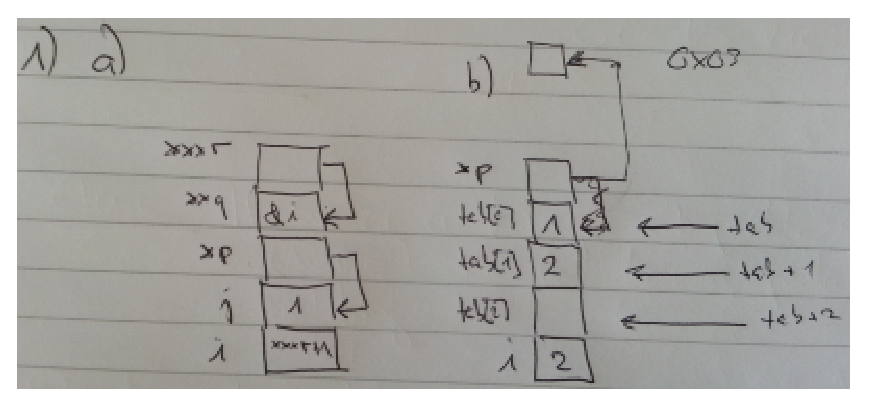
\includegraphics[scale=0.5]{eps/1a_b.eps} 
\caption{a) and b)}
\end{figure}

\begin{figure}[!htb]
\centering
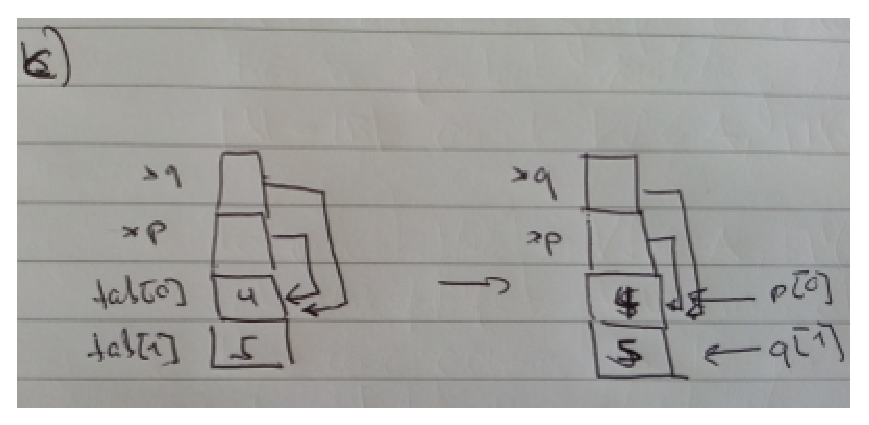
\includegraphics[scale=0.5]{eps/1c.eps} 
\caption{c)}
\end{figure}

\paragraph{Questions}
\subparagraph{a)}
\begin{enumerate}
\item q is of a type pointer to a int pointer.
\item \& i is the memory address of the variable i that can be assigned by the dereferenced operator *. The problem is that these pointer are incompatible types. The compiler will give a warning, so it compiles.
\end{enumerate}

\subparagraph{c)}
q is a pointer and not a name of an array. An array name can be used like a pointer. But a pointer that points to an array cannot be used like an array name.
Void pointer cannot be indexed. Thus we get a compile time error.

\subsection*{2. Pointers and Function arguments}

\begin{figure}[!htb]
\centering
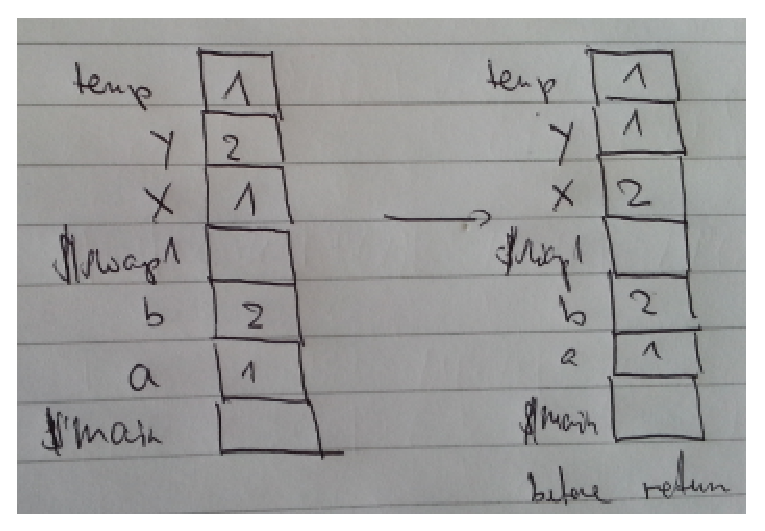
\includegraphics[scale=0.5]{eps/2_swap1.eps}  
\caption{swap1}
\end{figure}

\begin{figure}[!htb]
\centering
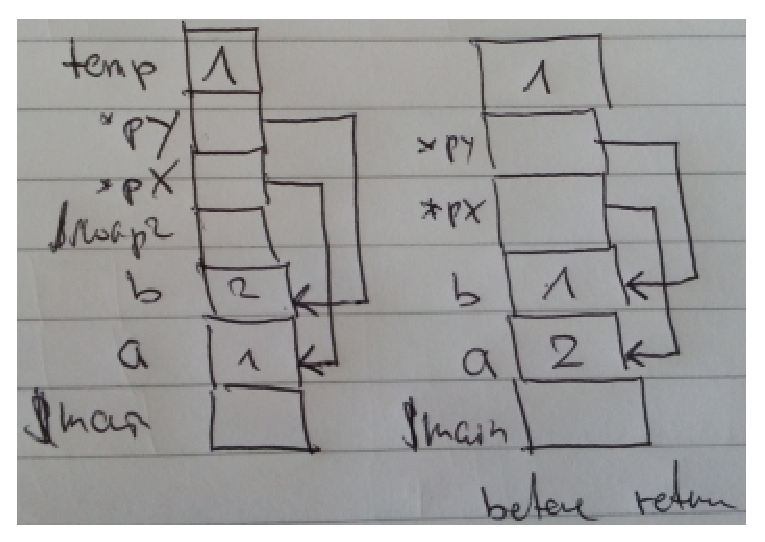
\includegraphics[scale=0.5]{eps/2_swap2.eps}  
\caption{swap2}
\end{figure}

\paragraph{Remark} 
I draw the picture in a wrong way!!! I pushed the function arguments in the wrong order. So px should be above px and x should be above y. 

\subsection*{3. About main(int argc, *argv[])}
\paragraph{1)} \quad

\begin{figure}[!htb]
\centering
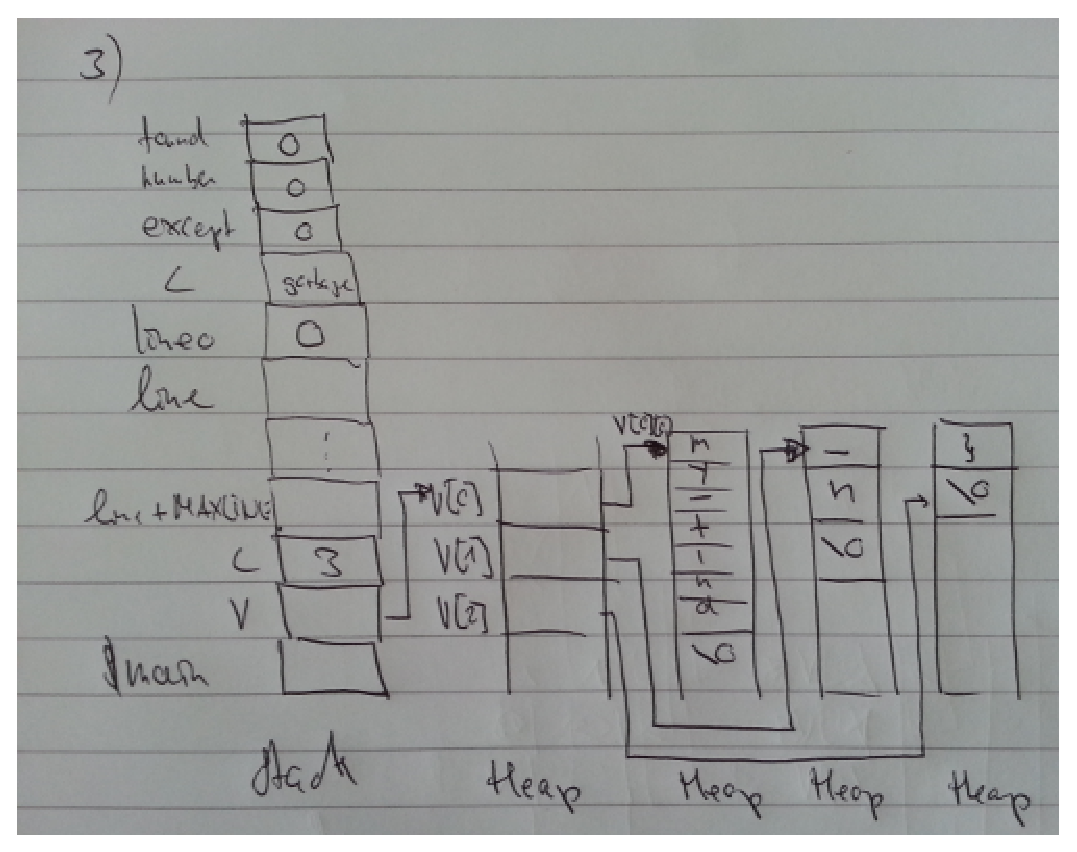
\includegraphics[scale=0.5]{eps/3.eps}  
\caption{my\_find}
\end{figure}

\paragraph{Question}
cat -n outputs all line and numbers them
my\_find produces the same result because the pattern is an empty char. Such an empty char occurs on each line therefore my\_find prints all lines.

\subsection*{4. About main(int argc, char* argv[])}
The modified version is given as follows:
\begin{lstlisting}
main(int argc, char *argv[])
{
    char line[MAXLINE];
    long lineno = 0;
    int c, i=0, except = 0, number = 0, found = 0;
    //orig: while (--argc > 0 && (*++argv)[0] == '-')
    while (--argc > 0 && argv[++i][0] == '-')
	while (c = *++argv[i]) //orig while (c = *++argv[0])
	    switch (c) {
		case 'x':
		    except = 1;
		    break;
		case 'n':
		    number = 1;
		    break;
		default:
		    printf("find: illegal option %c\n", c);
		    argc = 0;
		    found = -1;
		    break;
				}
    if (argc != 1)
	printf("Usage: find -x -n pattern\n");
    else
	while (_getline(line, MAXLINE) > 0) {
	    lineno++;
	    if ((strstr(line, argv[i]) != NULL) != except) {
		if (number)
		    printf("%ld:", lineno);
		printf("%s", line);
		found++;
	    }
	}
    return found;
}
\end{lstlisting}

\subsection*{5. Pointer to function }
\begin{figure}[!htb]
\centering
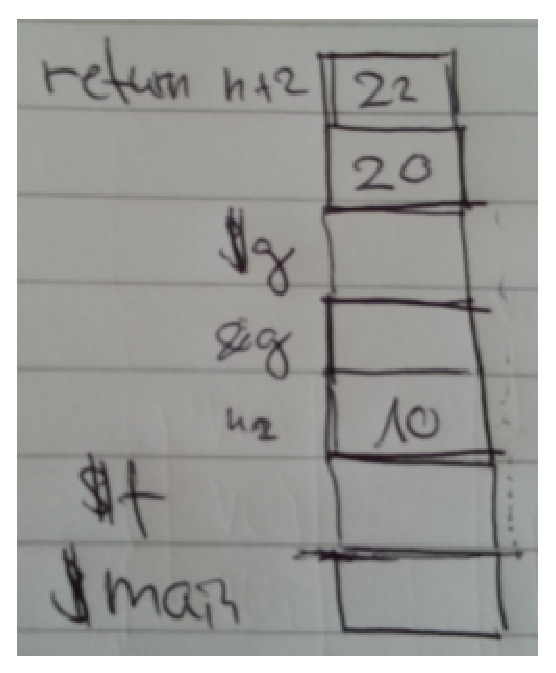
\includegraphics[scale=0.5]{eps/5.eps}  
\caption{my\_find}
\end{figure}

\subsection*{6. Stack and Fifo revisted}
\subsubsection*{a)}

\paragraph{Comparison Specf.h}
The difference are the function names. The stack implementation uses a stack as prefix and the queue fifo as prefix for the functions get and put. But basically both header files are identical in terms of the contract that the implementation must satisfy.

\paragraph{Comparison Test.c}
Basically there is no difference in both files besides the function names.
One minimal difference is the error treatment. In the fifo test file the first entry in the argv array is accessed in a printf statement.

\paragraph{Comparison Impl\_BA.c file}
Both files are similar except with some implementation details like tail, head and top etc.

\paragraph{Answer to the question}
As a first step I would write a generic header file "Collection.h" (like an interface) for different data structures like linked list, array list, stack, queue or hash table.
This header file would contain function prototypes like pop, put, get, add, first, last and remove.

Depending on the data structure not all operations must be implemented (we could use an empty implementation in some cases).

Besides that we could refactor the test program into a function which takes a list of function pointers that should be used.

We could pass the test program two arrays like this (pseudo):

\begin{lstlisting}
char ops[] = {'g','p'};
void fps[2] = {get,put};

test_program(ops,fps);
\end{lstlisting}

The identifier g belongs to get and p to put. 



\paragraph*{d)}
Such a function can be easily implemented as follows:
\begin{lstlisting}
int stack_size(){
	return top;
}
\end{lstlisting}

\end{document}